\section{绪论}\label{第1章-绪论}

\subsection{研究背景与意义}\label{1-1-研究背景与意义}

随着人口老龄化加剧，跌倒已成为 65 岁以上人群意外伤害死亡的首要原因\cite{ref1}。据世界卫生组织统计，全球每年约有 68 万人死于跌倒相关伤害\cite{ref2}。


智能跌倒检测系统能够在跌倒发生后第一时间发出告警，为急救争取宝贵时间。与人工看护相比，自动化检测系统具有全天候、低成本、覆盖范围广等优势，具有重要的应用价值。


\subsection{国内外研究现状}\label{1-2-国内外研究现状}

\subsubsection{基于视觉的方法}\label{1-2-1-基于视觉的方法}

基于视觉的跌倒检测方法利用摄像头采集的图像或视频信息进行分析。早期工作主要基于背景差分和光流估计\cite{ref3}，近年来深度学习方法取得了显著进展。


\subsubsection{基于传感器的方法}\label{1-2-2-基于传感器的方法}

惯性测量单元（IMU）因其低功耗、高采样率的特点被广泛应用于跌倒检测\cite{ref4}。加速度计和陀螺仪的组合能够有效捕捉运动加速度突变特征。


\subsection{本文研究内容}\label{1-3-本文研究内容}

本文的主要研究内容包括以下三个方面：


\begin{enumerate}[label=（\arabic*）]
  \item 构建多模态数据采集与预处理 pipeline，统一不同来源数据的时间戳对齐策略
  \item 设计跨模态注意力融合模块，实现 RGB、骨骼、IMU 三路特征的自适应加权
  \item 在公开数据集上进行系统评估，与主流基线方法进行对比实验
\end{enumerate}
\subsection{论文结构}\label{1-4-论文结构}

本文共分为五章。第 2 章介绍相关理论基础；第 3 章详细阐述所提方法；第 4 章报告实验结果；第 5 章总结全文并展望未来工作。


\section{相关理论基础}\label{第2章-相关理论基础}

\subsection{骨骼关键点估计}\label{2-1-骨骼关键点估计}

骨骼关键点估计是计算机视觉领域的基础任务，旨在从图像中定位人体关节位置。主流方法包括自顶向下（Top-Down）和自底向上（Bottom-Up）两类范式。


本文采用 OpenPose\cite{ref5} 提取 18 个关键点，包括颈部、肩部、肘部、腕部、髋部、膝部、踝部等关节，坐标归一化到 $[0, 1]$ 范围内。


\subsection{注意力机制}\label{2-2-注意力机制}

注意力机制（Attention Mechanism）最早由 Bahdanau 等人\cite{ref6}在神经机器翻译中提出，其核心思想是对输入序列中不同位置赋予不同权重。对于多模态融合，注意力权重可形式化为：


\[
\alpha\_i = \frac{\exp(e\_i)}{\sum\_{j=1}^{M} \exp(e\_j)}, \quad e\_i = f(h\_i)
\]


其中 $M$ 为模态数量，$h_i$ 为第 $i$ 个模态的特征向量，$f(\cdot)$ 为打分函数。


\subsection{多模态融合策略}\label{2-3-多模态融合策略}

多模态融合可在特征级（Feature-level）或决策级（Decision-level）进行。本文采用特征级融合，通过注意力权重对各模态特征进行加权求和，获得统一的融合表示。


\section{方法设计}\label{第3章-方法设计}

\subsection{整体框架}\label{3-1-整体框架}

如图所示，本文方法由三个特征提取分支和一个融合模块组成：


\begin{figure}[H]
  \centering
  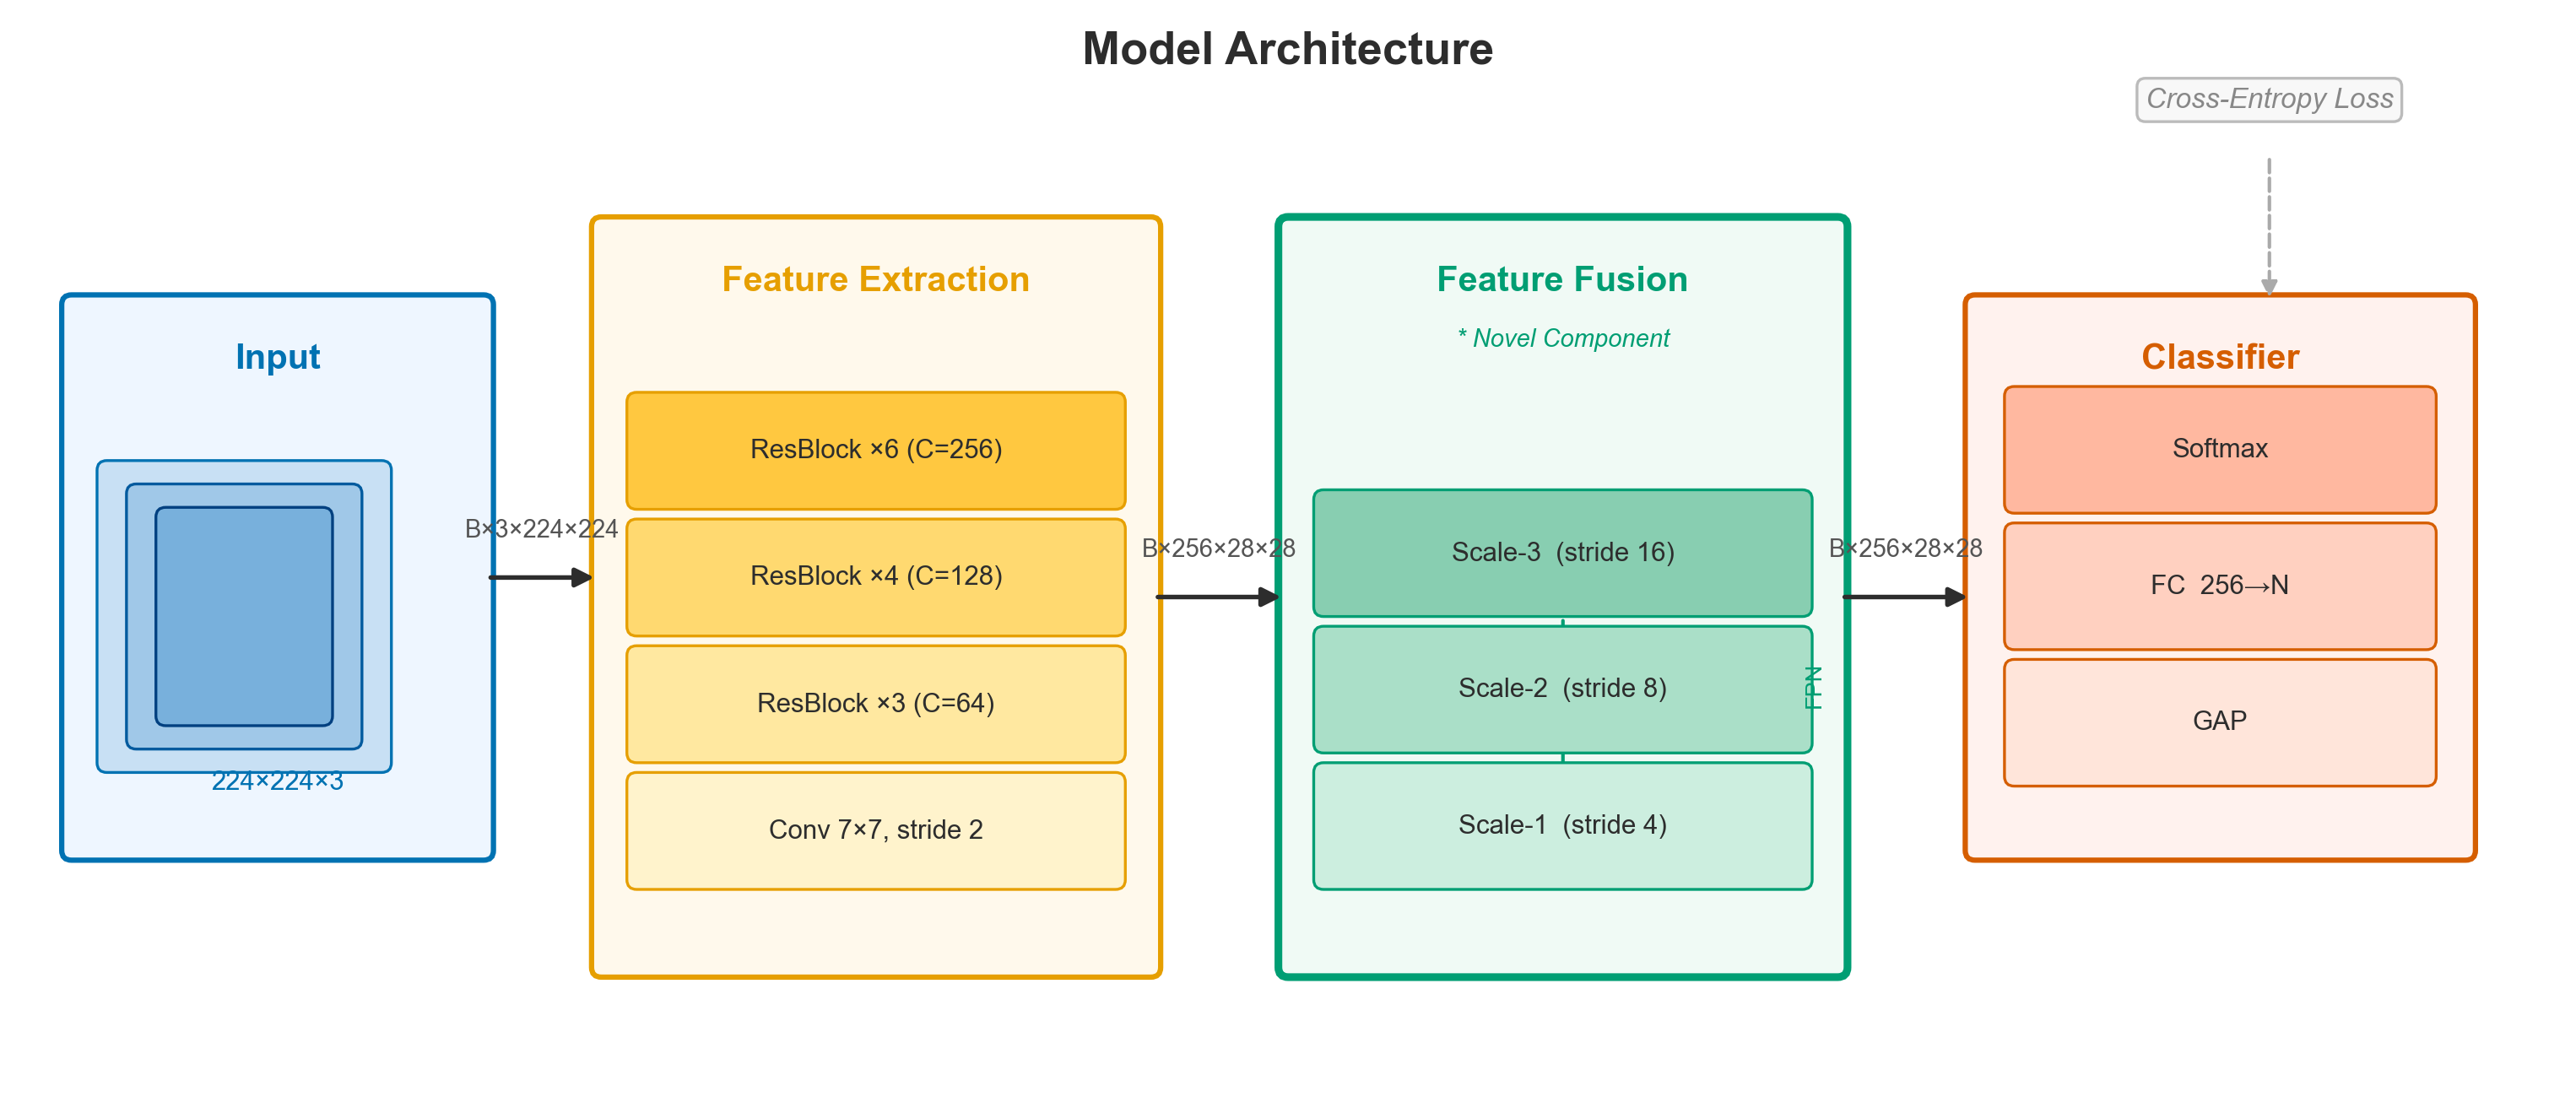
\includegraphics[width=0.88\textwidth]{Fig/fig_architecture.png}
  \caption{图3-1 多模态跌倒检测整体框架}
  \label{fig:图3-1-整体框架图}
\end{figure}

\begin{itemize}
  \item RGB 分支：基于 ResNet-50 提取空间外观特征
  \item 骨骼分支：基于图卷积网络（GCN）提取结构特征
  \item IMU 分支：基于 LSTM 提取时序动态特征
\end{itemize}
\subsection{跨模态注意力融合}\label{3-2-跨模态注意力融合}

设三路特征分别为 $\mathbf{f}_v \in \mathbb{R}^{512}$、$\mathbf{f}_s \in \mathbb{R}^{256}$、$\mathbf{f}_a \in \mathbb{R}^{128}$，经线性投影统一到 $d=256$ 维后，注意力融合计算如下：


\[
\mathbf{f}\_{fused} = \sum\_{i \in \{v,s,a\}} \alpha\_i \cdot \mathbf{W}\_i \mathbf{f}\_i
\]


其中权重 $\{\alpha_i\}$ 由 Softmax 归一化的打分函数给出。


\subsection{损失函数}\label{3-3-损失函数}

训练采用带类别权重的二分类交叉熵损失：


\[
\mathcal{L} = -\sum\_{n} \left[ w\_1 y\_n \log \hat{y}\_n + w\_0 (1-y\_n) \log(1-\hat{y}\_n) \right]
\]


\section{实验结果}\label{第4章-实验结果}

\subsection{数据集与实验设置}\label{4-1-数据集与实验设置}

本文在 UR Fall Detection\cite{ref7} 和 FDD\cite{ref8} 两个公开数据集上进行评估。数据集划分采用 7:1:2 的训练/验证/测试比例，使用 Adam 优化器，初始学习率 $1 \times 10^{-4}$，批大小 32。


\subsection{主要结果}\label{4-2-主要结果}

\noindent\textbf{表4-1 }


\begin{table}[H]
\centering
\begin{adjustbox}{max width=\linewidth}
\begin{tabular}{l|l|l|l|l}
\toprule
\textbf{方法} & \textbf{精确率} & \textbf{召回率} & \textbf{$F_1$} & \textbf{准确率} \\
\midrule
CNN-LSTM & 0.871 & 0.853 & 0.862 & 0.889 \\
ST-GCN & 0.884 & 0.876 & 0.880 & 0.901 \\
IMU-only & 0.862 & 0.841 & 0.851 & 0.878 \\
\textbf{本文方法} & \textbf{0.931} & \textbf{0.915} & \textbf{0.923} & \textbf{0.941} \\
\bottomrule
\end{tabular}
\end{adjustbox}
\end{table}

实验结果表明，本文方法在所有指标上均优于对比基线，$F_1$ 较最优基线提升了 4.3 个百分点。


\subsection{消融实验}\label{4-3-消融实验}

为验证各模态的贡献，进行消融实验，结果如下：


\noindent\textbf{表4-2 }


\begin{table}[H]
\centering
\begin{adjustbox}{max width=\linewidth}
\begin{tabular}{l|l|l}
\toprule
\textbf{配置} & \textbf{$F_1$} & \textbf{$\Delta F_1$} \\
\midrule
RGB only & 0.862 & — \\
+ 骨骼 & 0.891 & +0.029 \\
+ IMU & 0.905 & +0.043 \\
+ 注意力融合 & \textbf{0.923} & \textbf{+0.061} \\
\bottomrule
\end{tabular}
\end{adjustbox}
\end{table}

\section{总结与展望}\label{第5章-总结与展望}

\subsection{工作总结}\label{5-1-工作总结}

本文提出了一种基于多模态融合的跌倒检测方法，主要贡献包括：


\begin{enumerate}[label=（\arabic*）]
  \item 设计了跨模态注意力融合模块，实现三路异构特征的自适应整合
  \item 在两个公开数据集上验证了方法有效性，$F_1$ 达到 0.923
  \item 消融实验证明了注意力机制的必要性，单独去除任一模态均导致性能下降
\end{enumerate}
\subsection{未来展望}\label{5-2-未来展望}

未来工作将从以下方向继续探索：


\begin{itemize}
  \item 引入轻量化网络结构，降低边缘设备部署成本
  \item 扩展到多人场景的跌倒检测
  \item 研究隐私保护条件下的视频分析方案
\end{itemize}